\documentclass[a4paper,12pt]{article}
%\documentclass[a4paper,10pt]{scrartcl}

\usepackage[utf8]{inputenc}
\usepackage[english]{babel}
\usepackage[pdftex]{graphicx}
\usepackage{amssymb}
\usepackage{marvosym}
\usepackage{amsmath}
\usepackage{array}
\usepackage{geometry}

\geometry{verbose,tmargin=1cm,headheight=80pt,lmargin=2cm,bmargin=4cm,rmargin=2.5cm}

\title{Exercise 4 - Solution}
\author{}
\date{}

\pdfinfo{%
  /Title    ()
  /Author   ()
  /Creator  ()
  /Producer ()
  /Subject  ()
  /Keywords ()
}

\begin{document}
\maketitle

\section*{Task 4.1}
\begin{enumerate}
 \item \[\lambda = \frac{90^{\circ}}{2}= 45^{\circ}\]
 \[\eta = 90^{\circ} - \lambda - \varepsilon_{min} = 42^{\circ}\]
 \[\rho = arcsin\left(\frac{sin(\eta)}{cos(\varepsilon_{min})}\right) = 42.07^{\circ}\]
 \[h = r_E\left(\frac{1}{sin(\rho)}-1\right) = 3141km\]
 \item \[\lambda = \frac{90^{\circ}}{3}= 30^{\circ}\]
 \[\rho = 57.12^{\circ}\]
 \[h = 1217km\]
\end{enumerate}


\section*{Task 4.2}
given: $R_E = 6378km$, $\mu_E = 398600 \frac{km^3}{s^2}$, $h=900km$, $J_2 = 1082.63 \cdot 10^{-6}$, $\tau_e = 86164.10555+0.015C s$, $\tau_{s} = 3.155815\cdot10^7s$
\begin{enumerate}
 \item \[T = 2\pi\sqrt{\frac{a^3}{\mu_E}} = 2\pi\sqrt{\frac{(h+R_E)^3}{\mu_E}} = 6179.16s \]
 \[v = \sqrt{\frac{\mu_E}{a}} = \sqrt{\frac{\mu_E}{R_E + h}} = 7.40 \frac{km}{s}\]
 \item \[\Delta \Omega_{day} = 360^{\circ}\frac{\tau_e}{\tau_{s}} = 0.983 \frac{deg}{day}\]
 \[\Delta \Omega_{rev} = 360^{\circ}\frac{\tau_e}{\tau_{s}}\cdot \frac{T}{\tau_e} = 0.0705 \frac{deg}{rev}\]
 \[\Delta \Omega_{rev} = -\frac{3\pi J_2R_E^2}{a^2(1-\epsilon^2)^2}\cdot cos(i) \] circular orbit $\Rightarrow \epsilon$=0
 \[\Rightarrow i = arccos\bigg(-\frac{\Delta \Omega_{rev}a^2}{3\pi J_2R_E^2}\bigg) = 99.03^{\circ}\]
 
 \begin{figure}[!ht]
  \centering
  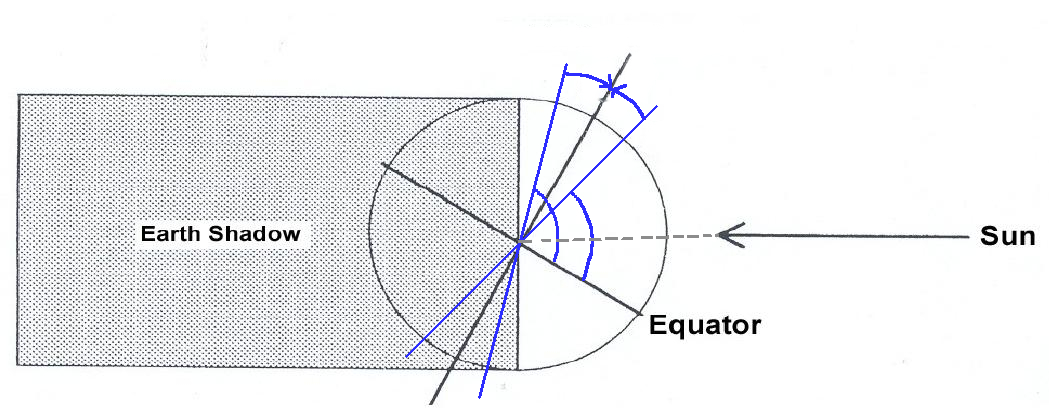
\includegraphics[scale=0.6]{../Loesungen/task4_2_}
 \end{figure}
\end{enumerate}
 \[\beta^* = arcsin(\frac{R_E}{R_E + h}) = 61.20^{\circ}\]
 \begin{itemize}
  \item orbit 1: \[\beta_1 = 90^{\circ} - 23.5^{\circ} + 9.03^{\circ} = 75.53^{\circ}\]
  \[\Rightarrow \beta_1 > \beta^* \Rightarrow \text{no eclipse} \]
  \item orbit 2: \[\beta_2 = 90^{\circ} - 23.5^{\circ} - 9.03^{\circ} = 57.53^{\circ}\]
  \[\Rightarrow \beta_2 < \beta^* \Rightarrow \text{eclipse} \]
 \end{itemize}
 \[F_e = \frac{1}{\pi}arccos\bigg(\frac{\sqrt{h^2 + 2R_Eh}}{(R_E + h)cos(\beta_2)}\bigg) = 0.1456 \approx 15\%\]
 \[T_{ecl} = T\cdot F_e = 14.99 min\]
 \vspace*{10pt}
 
 Both orbits will have an eclipse since the earth rotation axis stays fixed. The shadow periods of orbit 2 occur half a year later for orbit 1 which was 
 originally eclipse free.

\section*{Task 4.3}
given: $R_E = 6378km$, $\mu_E = 398600 \frac{km^3}{s^2}$, $J_2 = 1082.63\cdot 10^{-6}$, $i_e = 0^{\circ}$,$i = 53^{\circ}$
\begin{enumerate}
 \item \[T = 2\pi\sqrt{\frac{(R_E+h)^3}{\mu_E}} = 5801.07 s\]
 \[v = \sqrt{\frac{\mu_E}{(R_E + h)}} = 7.55 \frac{km}{s}\]
 \item \[\Delta \Omega = -\frac{3\pi J_2R_E^2}{(R_E +h)^2(1-\epsilon^2)^2}\cdot cos(i)\]
 a) circular orbit $\Rightarrow \epsilon$=0
 \[\Delta \Omega = -\frac{3\pi J_2R_E^2}{(R_E +h)^2}\cdot cos(i) = -0.00513 \frac{rad}{rev} = -0.076197 \frac{rad}{day}\]
 b) \[t_{ecl} = \frac{2\cdot \beta^*}{360^{\circ}} = \frac{2\cdot arcsin\left(\frac{r_E}{r_E+h}\right)}{360^{\circ}} = 2129.19s = 35.49min\]
 c) given: $r_a = (600+6378)km$, $r_b = (900+6378)km$
 \[\Delta v_1 = \sqrt{\frac{\mu_E}{r_a}}\bigg(\sqrt{\frac{2r_b}{r_a+r_b}}-1\bigg) = 0.07911\frac{km}{s}\]
 \[\Delta v_2 = \sqrt{\frac{\mu_E}{r_b}}\bigg(1-\sqrt{\frac{2r_a}{r_a+r_b}}\bigg) = 0.07828\frac{km}{s}\]
\end{enumerate}


\end{document}
